\chapter{Anhang}

Der Anhang enthält für das Verständnis einzelner Textstellen notwendige Dokumente.

\paragraph{zur Abbildung \ref{RTimeReport}:} Der Resolution Time Report zeigt auf, wann wie viel Zeit in Form von erledigter Task-Zeit pro Sprint erfüllt wurde. Dabei kann klar gesehen werden, dass desto weiter der Sprint vorangeschritten ist, umso mehr Zeit erfüllt wurde. Die Lücken zwischen den Datengipfeln lassen sich durch die im Januar liegende Praxisphase und die im Klausurenphase im sechsten Semester erklären.

\begin{figure}[ht]
\centering
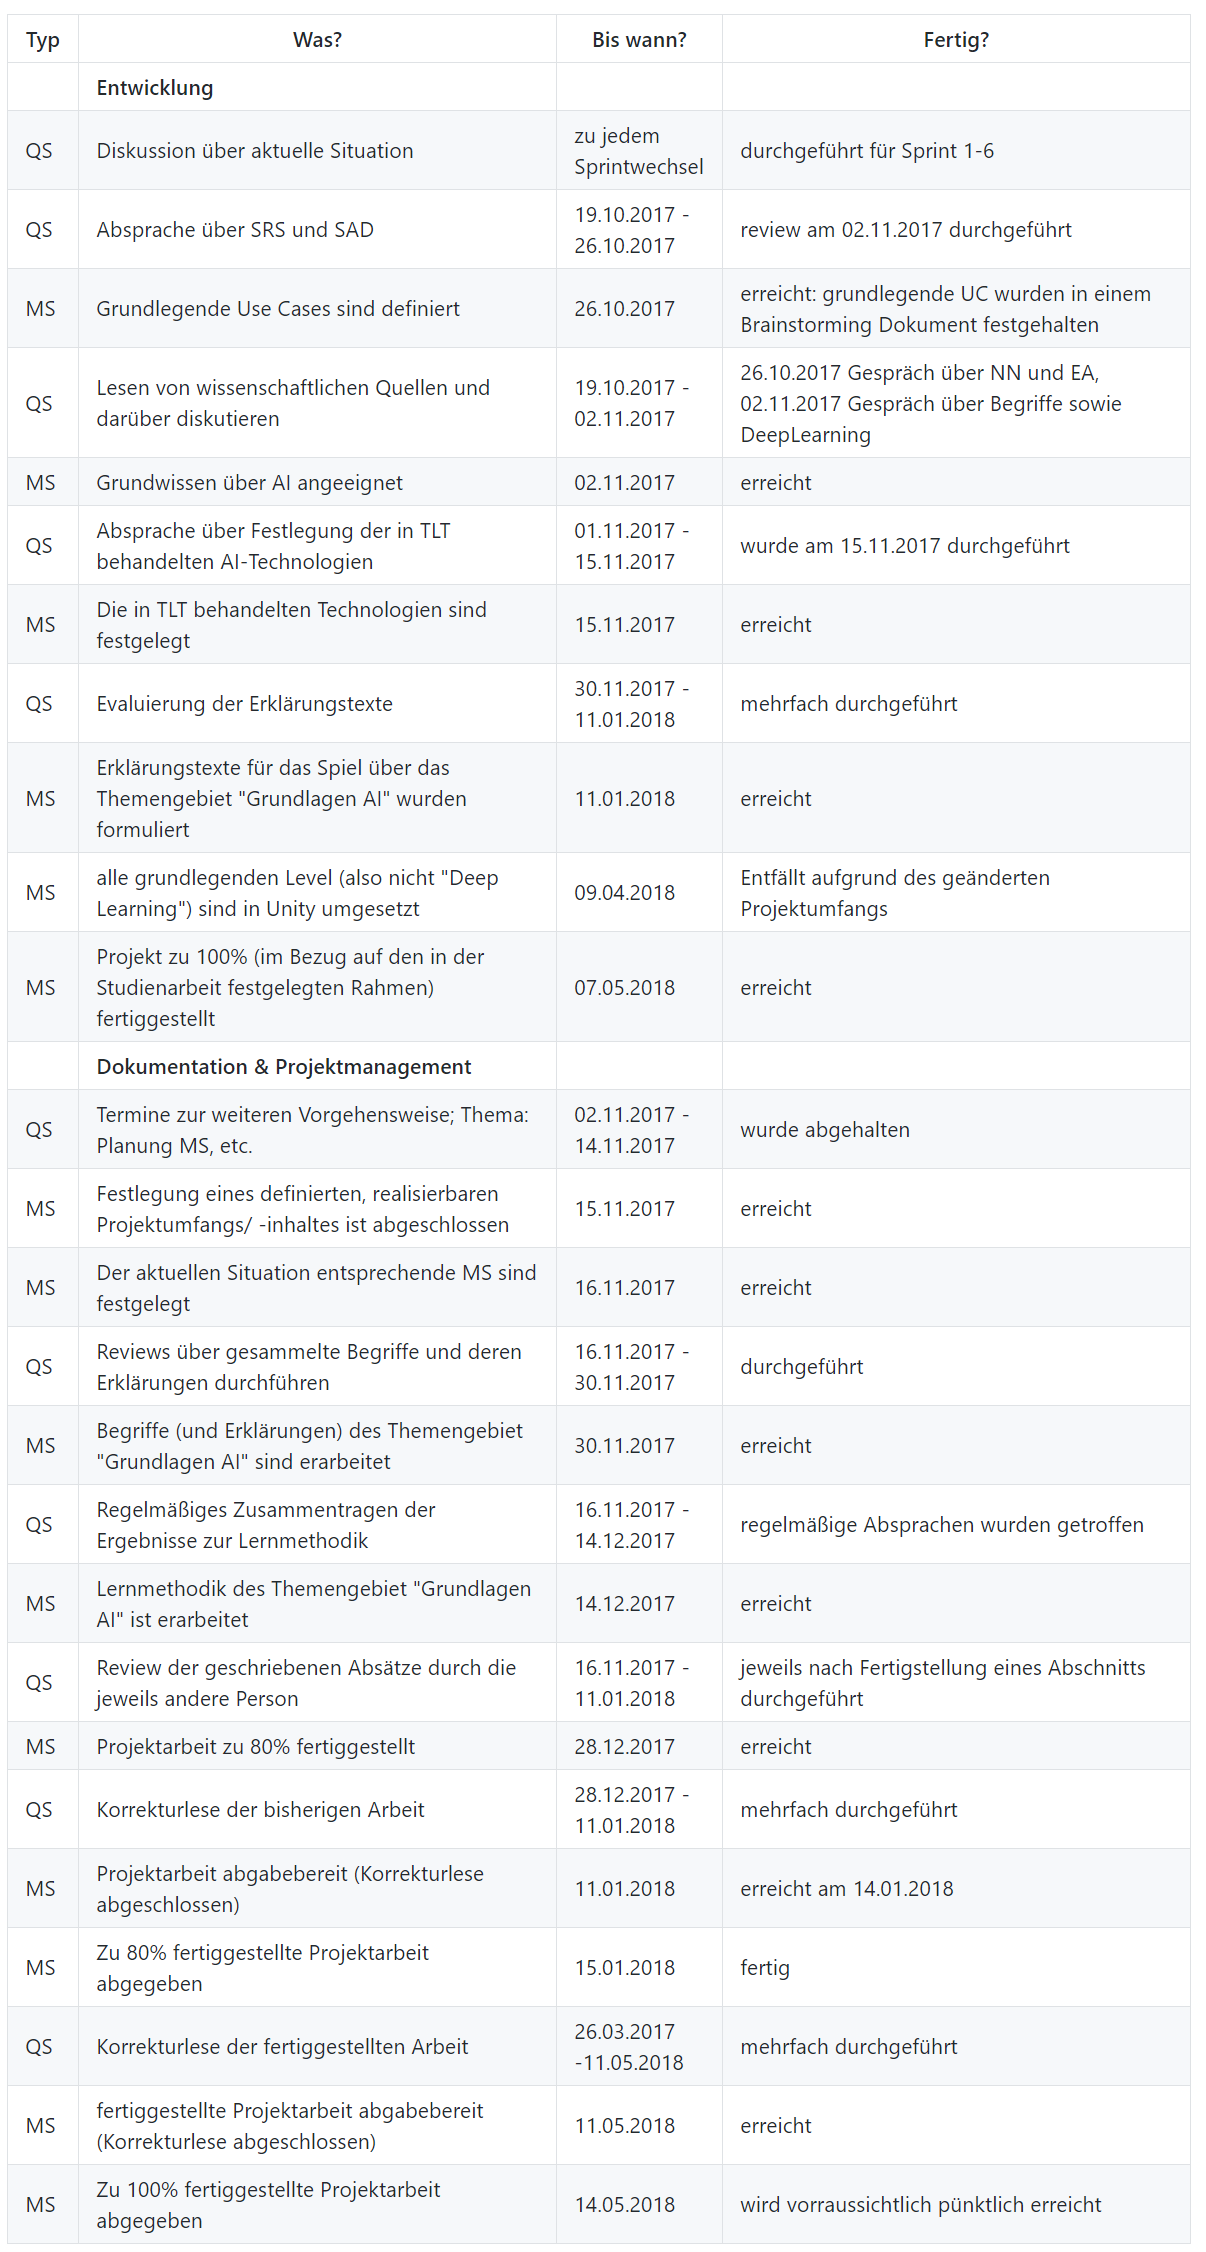
\includegraphics[scale=0.65]{bilder/QSMSS6.PNG}
\caption{QS und MS Analyse (Stand: 11.05.2018)}
\label{QSMSAnalyseBild}
\end{figure}

\begin{sidewaysfigure}[ht]
\centering
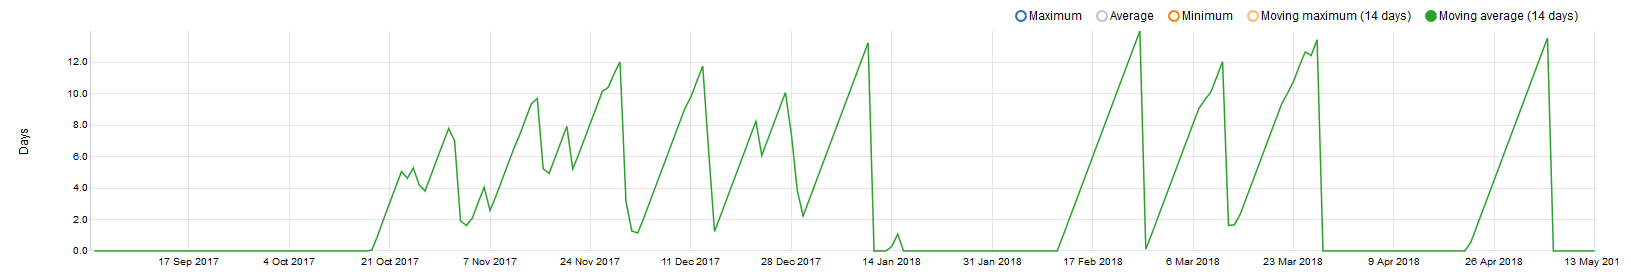
\includegraphics[scale=0.45]{bilder/ResoltutionTime.PNG}
\caption{Resolution Time Report (Stand: 13.05.2018)}
\label{RTimeReport}
\end{sidewaysfigure}

\begin{figure}[ht]
\centering
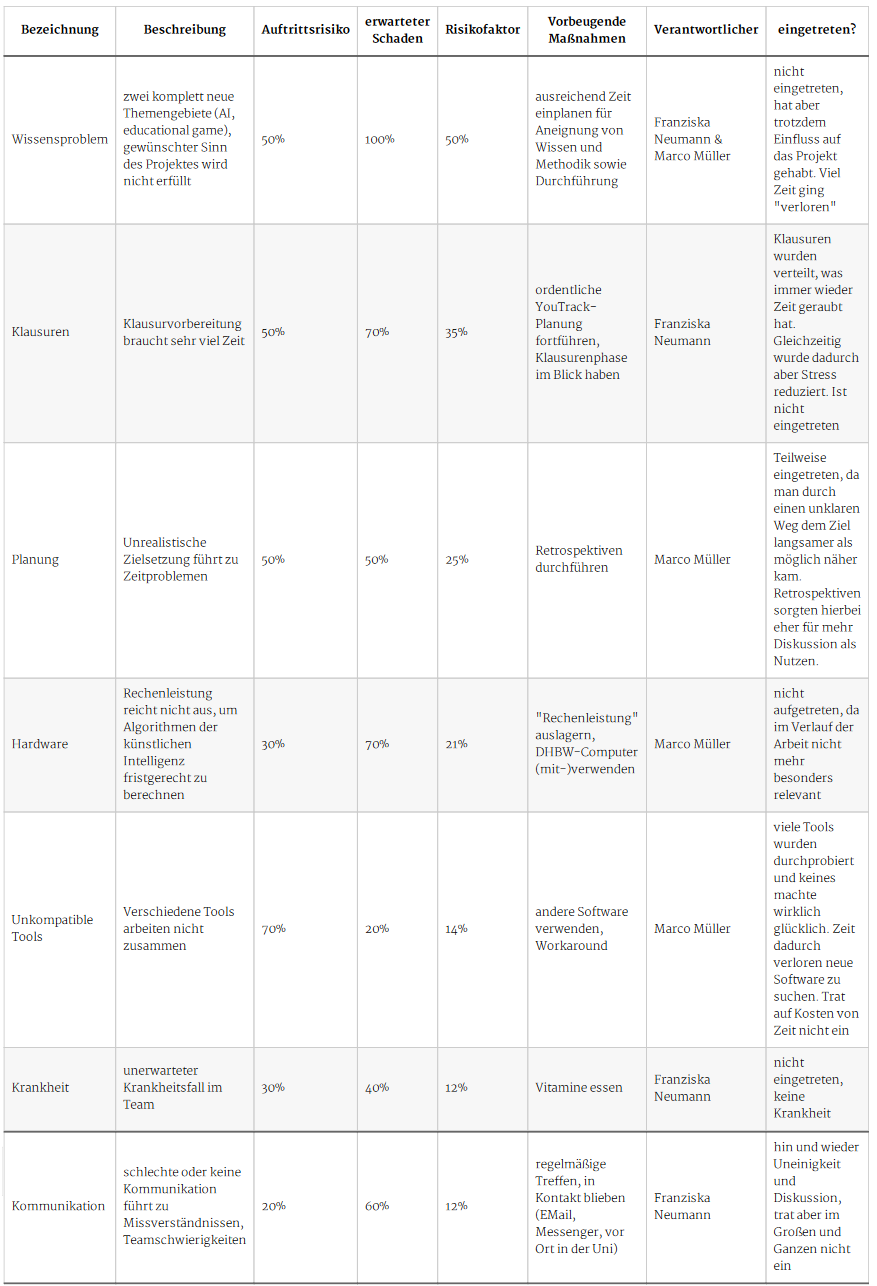
\includegraphics[scale=0.55]{bilder/RiskManagementTable.PNG}
\caption{Risk Management Table (Stand: 12.05.2018)}
\label{RiskManagementBild}
\end{figure}

\begin{sidewaysfigure}[ht]
\centering
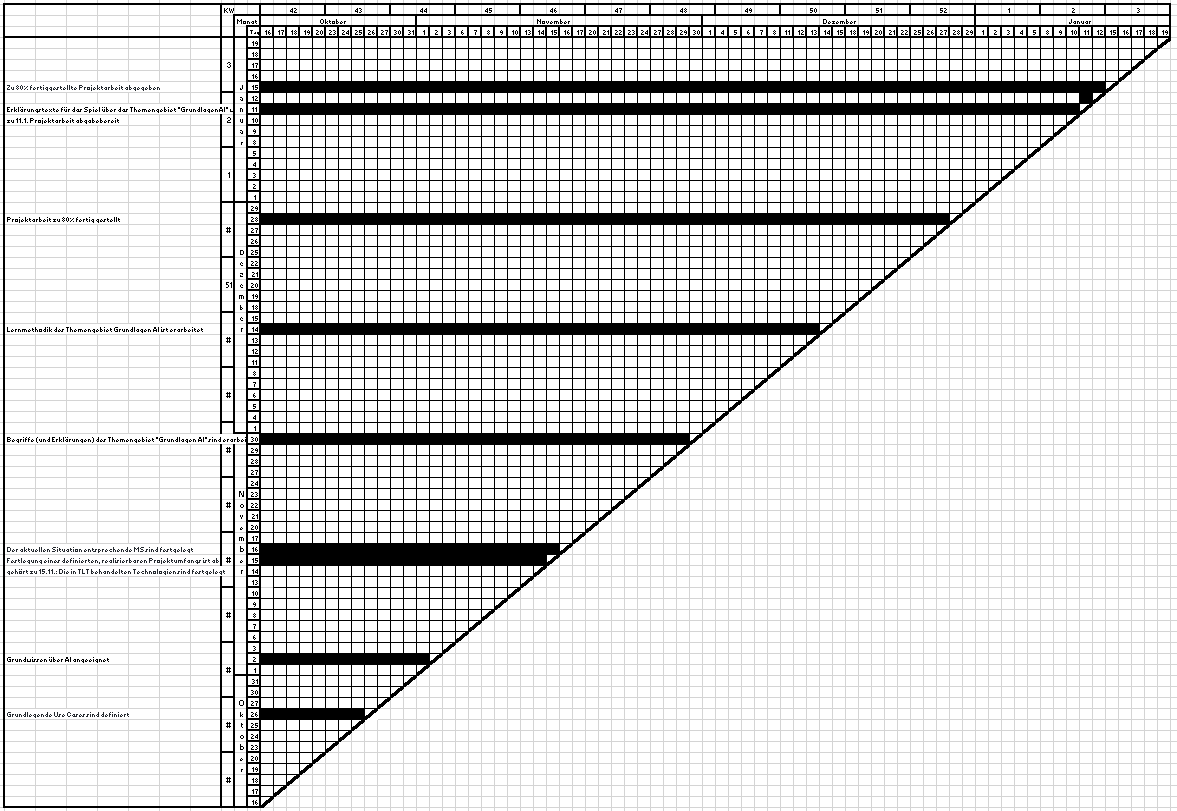
\includegraphics[scale=0.6]{bilder/MTA.PNG}
\caption{Meilenstein Trend Analyse (Stand: 14.01.2018)}
\label{MTA}
\end{sidewaysfigure}

\begin{sidewaysfigure}[ht]
\centering
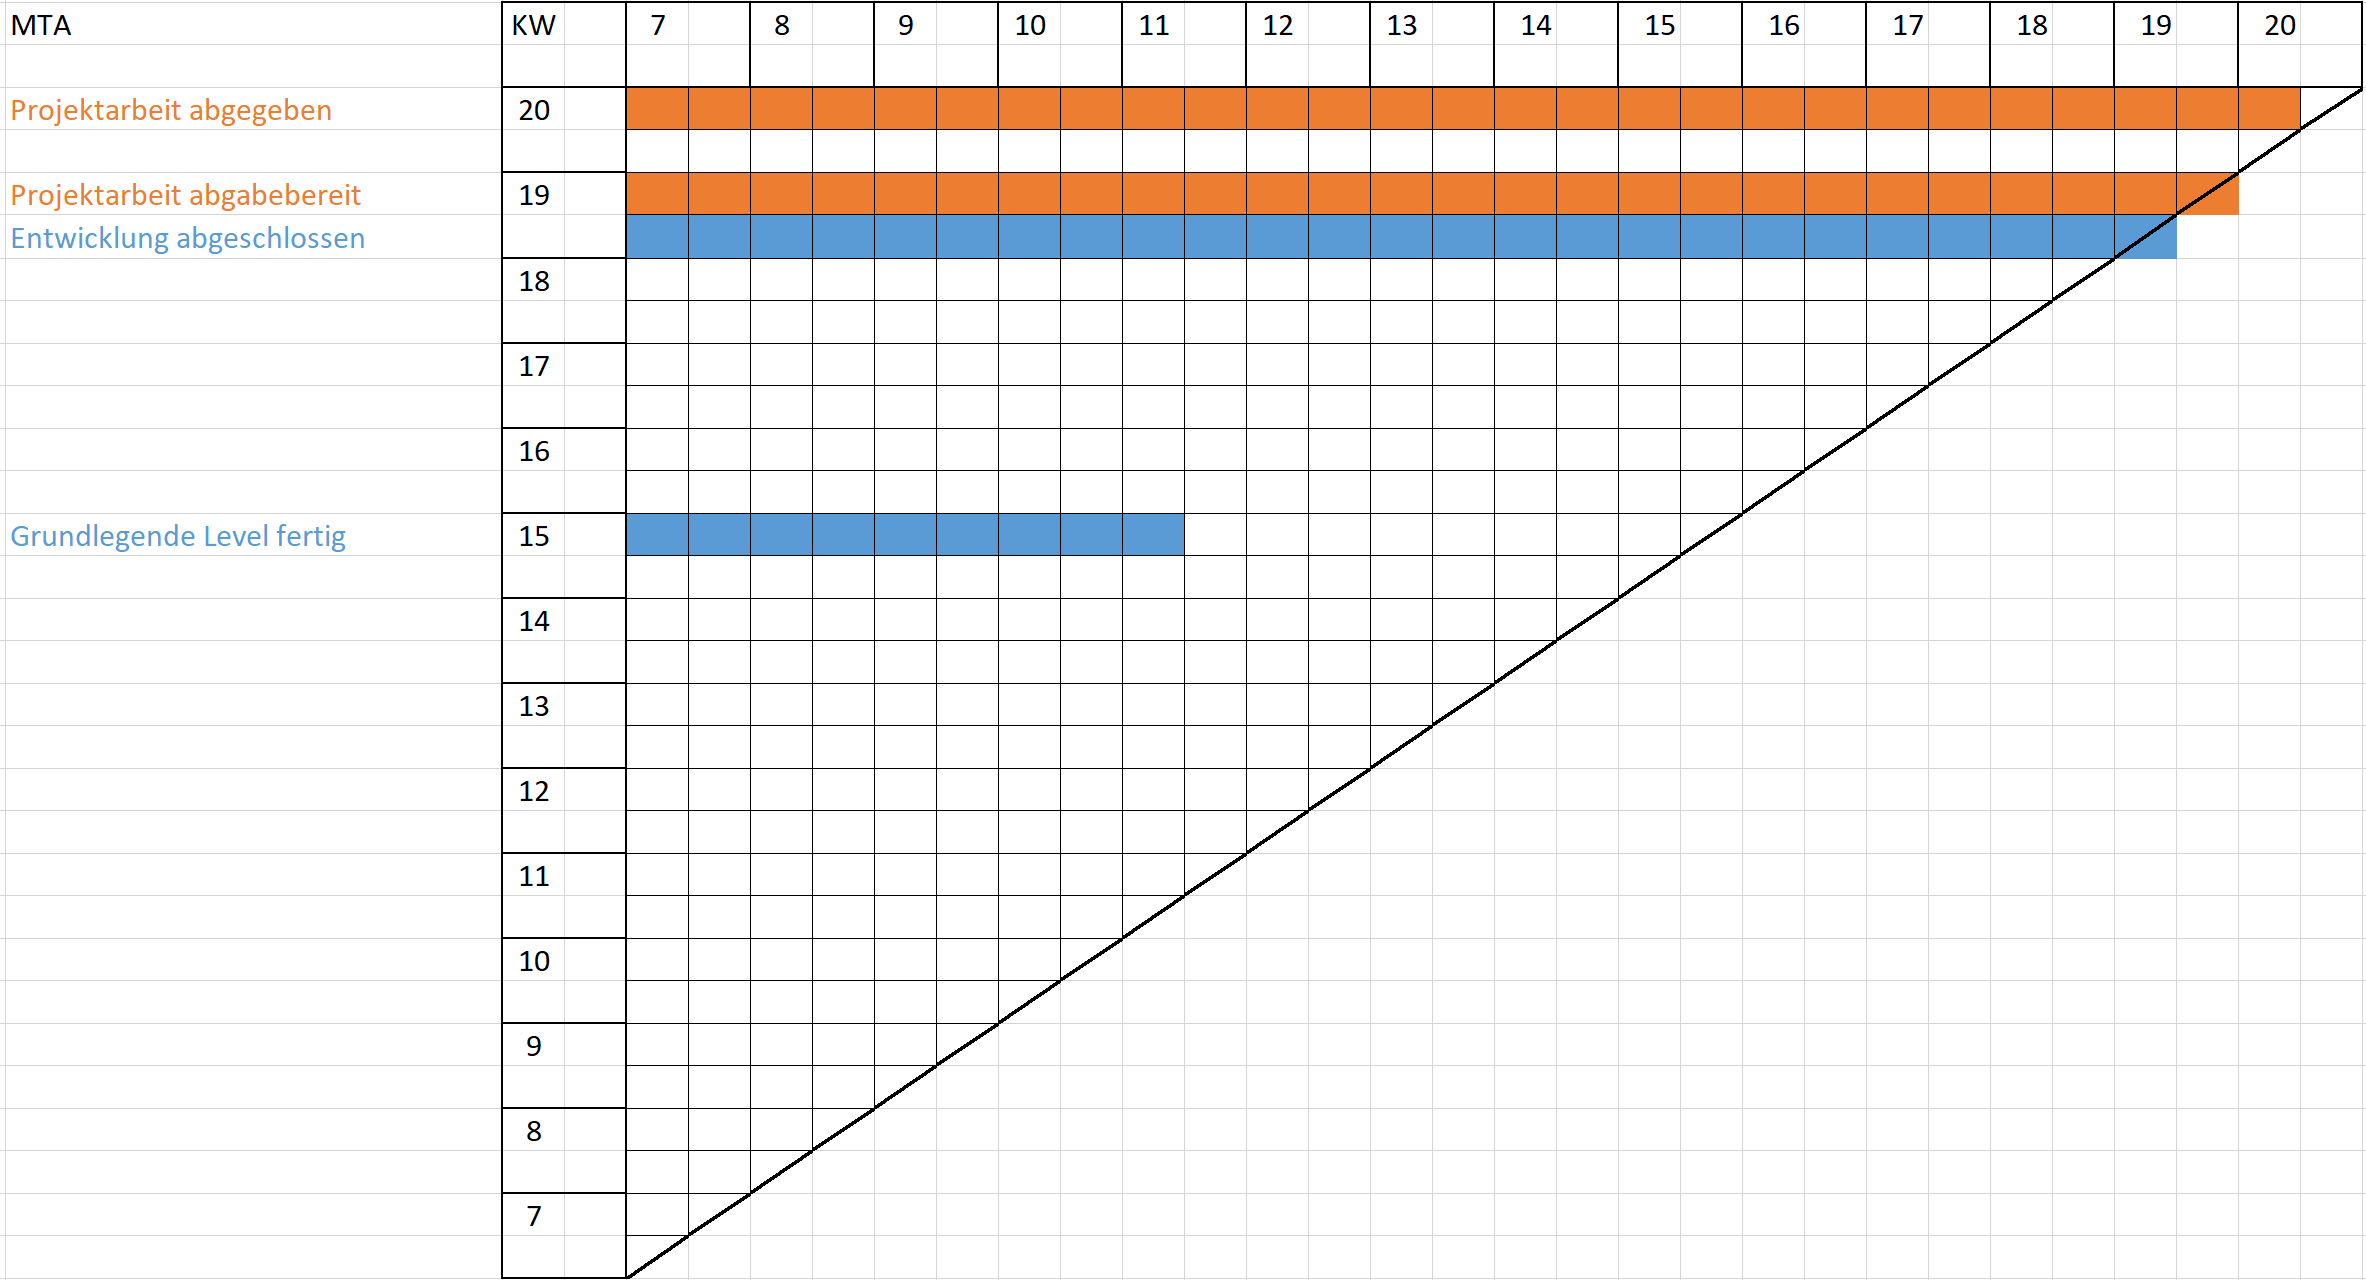
\includegraphics[scale=0.64]{bilder/MTAS6.PNG}
\caption{Meilenstein Trend Analyse (Stand: 11.05.2018)}
\label{MTA6}
\end{sidewaysfigure}